\section{Blazor Maui}
\label{sec:blazormaui}
Mit dem Release von .Net 6 kam auch der zusammenschluss von Blazor und .Net Maui erstmalig zum
Vorschein. Die Abkürzung \emph{Maui} steht dabei für \emph{Multi-platform Application UI}. Mit
Blazor Maui sollen Zukünftig Native Desktop oder Mobile Applikationen mit Blazor erstellt werden
können. Somit können nicht nur Native Applikationen mit hilfe von alt bekannten Html und Css
Komponenten erstellt werden, sondern auch schon erstellte Blazor Komponenten, die für eine
Webseite erstellt wurden, können wiederverwendet werden.
\newline
\newline
Die Architektur von Blazor Maui sieht vor, dass der Blazor code durch Maui in Nativen code
umgewandelt wird, um dann auf der jeweiligen Platform ausgeführt zu werden, wie im folgenden Bild
zu erkennen ist:

\begin{figure}[h]
    \centering
    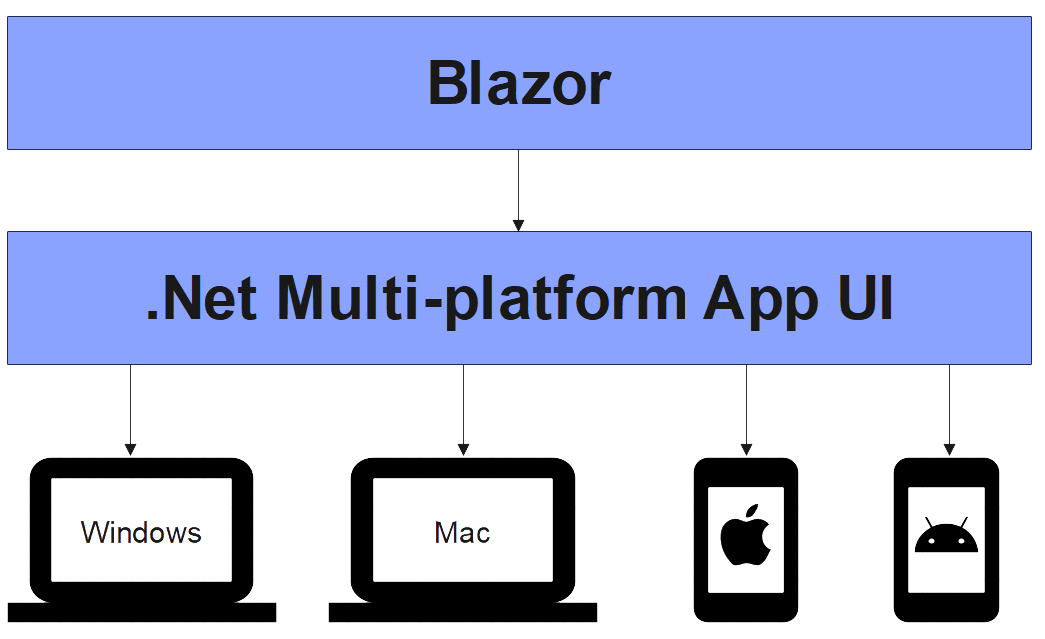
\includegraphics[width=\textwidth, center]{Blazor/BlazorMaui}
    \caption[Blazor Maui Architektur]{Blazor Maui Architektur}
    \label{img:BlazorMaui}
\end{figure}

Wie zu sehen ist, werden Windows, Mac, Ios und Android mithilfe von Maui untersützt, Linux
hingegen bleibt zu dem Zeitpunkt dieser Thesis noch außen vor.
\newline
\newline
Aufgrund dessen, das Linux zum derweiligen Zeitpunkt noch nicht unterstützt wird, und Open
Embedded System meist auf Linux basieren, wird Blazor Maui nicht weitergehend in dieser Thesis
behandelt.